\documentclass[thesis.tex]{subfiles}
\begin{document}
\selectlanguage{USenglish}
\chapter{Parameter Tuning}
\label{ch:eval1}

%\section{Tuning}
%\newglossaryentry{tuning}{name=Parameter tuning,text=parameter tuning,description={\nopostdesc}}
Not unlike other metaheuristics, our algorithms exhibit many parameters, meant for tuning them to specific problems. To allow for a fair comparison between the metaheuristics, these parameters ought to be \emph{tuned} first. In general, tuning a metaheuristic algorithm means to run it with different parameter settings, so as to find the best setting for a specific problem. A simple way to do that is by exhaustive search, which means invoking the algorithm with all possible combinations of all possible parameter values. Clearly, this does not scale; in the light of multiple parameters with large or even infinite sets of possible values, other methods seem more attractive. For this work, we facilitate an automatic parameter tuner called \gls{smac}, which uses regression models to describe the dependence of a target algorithm's performance on its parameter settings~\parencite{smac}.%
%\footnote{Other tuners that have been considered are ParamILS~\parencite{paramils-paper}, which seems deprecated in favor of \gls{smac}, and irace~\parencite{irace-paper}.}
Given a set of instances for training, \gls{smac} returns the best-performing parameter configuration it can heuristically find. Somewhat arbitrarily, a runtime limit of 1000 seconds has been imposed on each run during the tuning process, which represents a trade-off between the solution quality of an individual run and the solution quality of the parameter tuning (assuming that the overall runtime should not exceed a few weeks).

The training instances that have been considered in this work are 79 Graph Coloring instances, most of which stem from the Second \gls{DIMACS} Implementation Challenge\footnote{The Second \gls{DIMACS} Implementation Challenges been concerned with the $\NP$ hard problems Maximum Clique, Graph Coloring, and Satisfiability, and has been organized between 1992 and 1993.}~\parencite{dimacs-challenges}. The instances may be obtained, for instance, from~\parencite{graph-coloring-instances}.

%\subsection[Training Set]{Training Set: Instances Used for Tuning}
Tables \ref{training-set-DSJ} to \ref{training-set-LAT} on pages \pageref{training-set-DSJ}--\pageref{training-set-LAT} show the instances of the training set. They list all instances of the respective category, along with the instance's number of vertices (|V|) and edges (|E|). Additionally, the number of samples gathered during parameter tuning is given, with the instance that has been involved in the most evaluations given in bold typeface.

%\newcommand{\InstanceDescription}[5]{\vspace{\baselineskip}\begin{minipage}{\textwidth}\textbf{#1}\hfill by #2 (#3)\\[.2\baselineskip plus 0pt minus 0pt]\noindent{#4}\begin{center}#5\end{center}\end{minipage}}
%\newcommand{\InstanceDescription}[5]{\vspace{\baselineskip}\begin{minipage}{\textwidth}\hfill by #2 (#3)\\[.2\baselineskip plus 0pt minus 0pt]\noindent{#4}\begin{center}#5\end{center}\end{minipage}}
%\newcommand{\InstanceDescription}[5]{\vspace{\baselineskip}\begin{minipage}{\textwidth}\noindent{#4}. By #2.\begin{center}#5\end{center}\end{minipage}}
\newcommand{\InstanceDescription}[5]{%
   % #1: Instance Category
   % #2: Author Fullname
   % #3: Author eMail
   % #4: Description
   % #5: Table
   %\begin{sidefigure}{toc={Training Set, #1 Instances},caption={#4},label={training-set-#1}}#5\end{sidefigure}}
   \begin{table}[htbp]\caption[Training Set, #1 Instances]{#4}\label{training-set-#1}\centering\small{#5}\end{table}}
\InstanceDescription{DSJ}{David Johnson}{dsj@research.att.com}{%
Random graphs used in his paper with Aragon, McGeoch, and Schevon, \enquote{Optimization by Simulated Annealing: An Experimental Evaluation; Part II, Graph Coloring and Number Partitioning}, Operations Research, 31, 378--406 (1991). DSJC are standard $(n,p)$ random graphs. DSJR are geometric graphs, and DSJR*.c complements of geometric graphs}{%
\begin{tabularx}{.8\textwidth}{XS[table-format=4]S[table-format=6]S[table-format=2]S[table-format=2]S[table-format=2]} \toprule
   &&&\multicolumn{3}{c}{\header{Number of Samples}}\\\cmidrule{4-6}
   \header{Instance Name} & \header{|V|} & \header{|E|} & \header{\gls{MA1}} & \header{\gls{MA2}} & \header{\gls{MA3}} \\\midrule
\Instance{DSJC125.1}                                         &  125 &   1472 & 17 & 24 & 19 \\
\Instance{DSJC125.5}                                         &  125 &   7782 & 18 & 22 & 19 \\
\Instance{DSJC125.9}                                         &  125 &  13922 & 16 & 23 & 29 \\
\Instance{DSJC250.1}                                         &  250 &   6436 & 21 & 18 & 17 \\
\Instance{DSJC250.5}                                         &  250 &  31336 & 25 & 30 & 22 \\
\Instance{DSJC250.9}                                         &  250 &  55794 & 30 & 24 & 29 \\
\Instance{DSJC500.1}                                         &  500 &  24916 & 14 & 16 & 16 \\
\Instance{DSJC500.5}                                         &  500 & 125248 & 24 & 19 & 25 \\
\textbf{\Instance{DSJC500.9}}                                &  500 & 224874 & 30 & \boldentry{2}{31} & 28 \\
\Instance{DSJC1000.1}                                        & 1000 &  99258 & 17 & 17 & 19 \\
\Instance{DSJC1000.5}                                        & 1000 & 499652 & 23 & 25 & 15 \\
\textbf{\Instance{DSJC1000.9}}                               & 1000 & 898898 & \boldentry{2}{31} & 34 & 26 \\
\Instance{DSJR500.1}                                         &  500 &   7110 & 20 & 22 & 14 \\
\textbf{\Instance{DSJR500.1c}}                               &  500 & 242550 & 29 & 32 & \boldentry{2}{39} \\
\Instance{DSJR500.5}                                         &  500 & 117724 & 21 & 15 & 18 \\
   \bottomrule
\end{tabularx}
}

\InstanceDescription{CUL}{Joe Culberson}{joe@cs.ualberta.ca}{%
Quasi-random coloring problem}{%
\begin{tabularx}{.8\textwidth}{XS[table-format=4]S[table-format=6]S[table-format=2]S[table-format=2]S[table-format=2]} \toprule
   &&&\multicolumn{3}{c}{\header{Number of Samples}}\\\cmidrule{4-6}
   \header{Instance Name} & \header{|V|} & \header{|E|} & \header{\gls{MA1}} & \header{\gls{MA2}} & \header{\gls{MA3}} \\\midrule
\Instance{flat300\textunderscore{}20\textunderscore{}0}      &  300 &  21375 & 21 & 26 & 26 \\
\textbf{\Instance{flat300\textunderscore{}26\textunderscore{}0}} &  300 &  21633 & \boldentry{2}{30} & 21 & \boldentry{2}{32} \\
\Instance{flat300\textunderscore{}28\textunderscore{}0}      &  300 &  21695 & 16 & 16 & 20 \\
\Instance{flat1000\textunderscore{}50\textunderscore{}0}     & 1000 & 245000 & 21 & 19 & 21 \\
\Instance{flat1000\textunderscore{}60\textunderscore{}0}     & 1000 & 245830 & 24 & 19 & 22 \\
\textbf{\Instance{flat1000\textunderscore{}76\textunderscore{}0}} & 1000 & 246708 & 27 & \boldentry{2}{32} & 22 \\
   \bottomrule
\end{tabularx}
}

\InstanceDescription{LAT}{Gary Lewandowski}{lewandow@cs.wisc.edu}{%
Latin square problem}{%
\begin{tabularx}{.8\textwidth}{XS[table-format=4]S[table-format=6]S[table-format=2]S[table-format=2]S[table-format=2]} \toprule
   &&&\multicolumn{3}{c}{\header{Number of Samples}}\\\cmidrule{4-6}
   \header{Instance Name} & \header{|V|} & \header{|E|} & \header{\gls{MA1}} & \header{\gls{MA2}} & \header{\gls{MA3}} \\\midrule
\textbf{\Instance{latin\textunderscore{}square\textunderscore{}10}} &  900 & 307350 & \boldentry{2}{25} & \boldentry{2}{20} & \boldentry{2}{26} \\
   \bottomrule
\end{tabularx}
}

\InstanceDescription{REG}{Gary Lewandowski}{gary@cs.wisc.edu}{%
Problem based on register allocation for variables in real codes}{%
\begin{tabularx}{.8\textwidth}{XS[table-format=4]S[table-format=6]S[table-format=2]S[table-format=2]S[table-format=2]} \toprule
   &&&\multicolumn{3}{c}{\header{Number of Samples}}\\\cmidrule{4-6}
   \header{Instance Name} & \header{|V|} & \header{|E|} & \header{\gls{MA1}} & \header{\gls{MA2}} & \header{\gls{MA3}} \\\midrule
\Instance{fpsol2.i.1}                                        &  496 &  11654 & 18 & 23 & 18 \\
\textbf{\Instance{fpsol2.i.2}}                               &  451 &   8691 & \boldentry{2}{24} & 21 & 18 \\
\textbf{\Instance{fpsol2.i.3}}                               &  425 &   8688 & 21 & \boldentry{2}{24} & \boldentry{2}{27} \\
\Instance{inithx.i.1}                                        &  864 &  18707 & 17 & 20 & 18 \\
\Instance{inithx.i.2}                                        &  645 &  13979 & 15 & 20 & 21 \\
\textbf{\Instance{inithx.i.3}}                               &  621 &  13969 & \boldentry{2}{25} & \boldentry{2}{30} & \boldentry{2}{25} \\
\textbf{\Instance{mulsol.i.1}}                               &  197 &   3925 & 24 & 24 & \boldentry{2}{33} \\
\textbf{\Instance{mulsol.i.2}}                               &  188 &   3885 & \boldentry{2}{33} & \boldentry{2}{33} & 22 \\
\Instance{mulsol.i.3}                                        &  184 &   3916 & 22 & 20 & 19 \\
\Instance{mulsol.i.4}                                        &  185 &   3946 & 20 & 19 & 24 \\
\Instance{mulsol.i.5}                                        &  186 &   3973 & 22 & 18 & 20 \\
\Instance{zeroin.i.1}                                        &  211 &   4100 & 20 & 20 & 21 \\
\Instance{zeroin.i.2}                                        &  211 &   3541 & 23 & 19 & 16 \\
\textbf{\Instance{zeroin.i.3}}                               &  206 &   3540 & \boldentry{2}{35} & \boldentry{2}{27} & \boldentry{2}{31} \\
   \bottomrule
\end{tabularx}
}

\InstanceDescription{LEI}{Craig Morgenstern}{morgenst@riogrande.cs.tcu.edu}{%
Leighton graphs with guaranteed coloring size. A reference is F.T.\@ Leighton, Journal of Research of the National Bureau of Standards, 84: 489--505 (1979)}{%
\begin{tabularx}{.8\textwidth}{XS[table-format=4]S[table-format=6]S[table-format=2]S[table-format=2]S[table-format=2]} \toprule
   &&&\multicolumn{3}{c}{\header{Number of Samples}}\\\cmidrule{4-6}
   \header{Instance Name} & \header{|V|} & \header{|E|} & \header{\gls{MA1}} & \header{\gls{MA2}} & \header{\gls{MA3}} \\\midrule
\Instance{le450\textunderscore{}5a}                          &  450 &   5714 & 23 & 20 & 29 \\
\Instance{le450\textunderscore{}5b}                          &  450 &   5734 & 23 & 24 & 19 \\
\textbf{\Instance{le450\textunderscore{}5c}}                 &  450 &   9803 & 28 & \boldentry{2}{31} & 30 \\
\Instance{le450\textunderscore{}5d}                          &  450 &   9757 & 21 & 18 & 23 \\
\Instance{le450\textunderscore{}15a}                         &  450 &   8168 & 17 & 21 & 18 \\
\Instance{le450\textunderscore{}15b}                         &  450 &   8169 & 17 & 21 & 20 \\
\textbf{\Instance{le450\textunderscore{}15c}}                &  450 &  16680 & \boldentry{2}{38} & 29 & \boldentry{2}{34} \\
\Instance{le450\textunderscore{}15d}                         &  450 &  16750 & 13 & 24 & 24 \\
\Instance{le450\textunderscore{}25a}                         &  450 &   8260 & 16 & 14 & 22 \\
\Instance{le450\textunderscore{}25b}                         &  450 &   8263 & 19 & 24 & 22 \\
\Instance{le450\textunderscore{}25c}                         &  450 &  17343 & 23 & 25 & 20 \\
\Instance{le450\textunderscore{}25d}                         &  450 &  17425 & 16 & 19 & 13 \\
   \bottomrule
\end{tabularx}
}

\InstanceDescription{SGB1}{Michael Trick}{trick@cmu.edu}{%
Book Graphs from Donald Knuth's Stanford GraphBase. Given a work of literature, a graph is created where each node represents a character. Two nodes are connected by an edge if the corresponding characters encounter each other in the book. Knuth creates the graphs for five classic works: Tolstoy's Anna Karenina (anna), Dicken's David Copperfield (david), Homer's Iliad (homer), Twain's Huckleberry Finn (huck), and Hugo's Les Mis\'erables (jean)}{%
\begin{tabularx}{.8\textwidth}{XS[table-format=4]S[table-format=6]S[table-format=2]S[table-format=2]S[table-format=2]} \toprule
   &&&\multicolumn{3}{c}{\header{Number of Samples}}\\\cmidrule{4-6}
   \header{Instance Name} & \header{|V|} & \header{|E|} & \header{\gls{MA1}} & \header{\gls{MA2}} & \header{\gls{MA3}} \\\midrule
\textbf{\Instance{anna}}                                     &  138 &    986 & \boldentry{2}{31} & 25 & 15 \\
\Instance{david}                                             &   87 &    812 & 25 & 17 & 17 \\
\Instance{homer}                                             &  561 &   3258 & 18 & 31 & 23 \\
\Instance{huck}                                              &   74 &    602 & 20 & 27 & 32 \\
\textbf{\Instance{jean}}                                     &   80 &    508 & 30 & \boldentry{2}{35} & \boldentry{2}{37} \\
   \bottomrule
\end{tabularx}
}

\InstanceDescription{SGB2}{Michael Trick}{trick@cmu.edu}{%
Game Graph from Donald Knuth's Stanford GraphBase. A graph representing the games played in a college football season can be represented by a graph where the nodes represent each college team. Two teams are connected by an edge if they played each other during the season. Knuth gives the graph for the 1990 college football season}{%
\begin{tabularx}{.8\textwidth}{XS[table-format=4]S[table-format=6]S[table-format=2]S[table-format=2]S[table-format=2]} \toprule
   &&&\multicolumn{3}{c}{\header{Number of Samples}}\\\cmidrule{4-6}
   \header{Instance Name} & \header{|V|} & \header{|E|} & \header{\gls{MA1}} & \header{\gls{MA2}} & \header{\gls{MA3}} \\\midrule
\textbf{\Instance{games120}}                                 &  120 &   1276 & \boldentry{2}{23} & \boldentry{2}{22} & \boldentry{2}{21} \\
   \bottomrule
\end{tabularx}
}

\InstanceDescription{SGB3}{Michael Trick}{trick@cmu.edu}{%
Miles Graphs from Donald Knuth's Stanford GraphBase. These graphs are similar to geometric graphs in that nodes are placed in space with two nodes connected if they are close enough. These graphs, however, are not random. The nodes represent a set of United States cities and the distance between them is given by by road mileage from 1947. These graphs are also due to Kuth}{%
\begin{tabularx}{.8\textwidth}{XS[table-format=4]S[table-format=6]S[table-format=2]S[table-format=2]S[table-format=2]} \toprule
   &&&\multicolumn{3}{c}{\header{Number of Samples}}\\\cmidrule{4-6}
   \header{Instance Name} & \header{|V|} & \header{|E|} & \header{\gls{MA1}} & \header{\gls{MA2}} & \header{\gls{MA3}} \\\midrule
\Instance{miles250}                                          &  128 &    774 & 15 & 18 & 19 \\
\textbf{\Instance{miles500}}                                 &  128 &   2340 & \boldentry{2}{26} & 23 & \boldentry{2}{23} \\
\Instance{miles750}                                          &  128 &   4226 & 21 & 23 & 22 \\
\textbf{\Instance{miles1000}}                                &  128 &   6432 & 26 & \boldentry{2}{28} & 21 \\
\Instance{miles1500}                                         &  128 &  10396 & 22 & 23 & 23 \\
   \bottomrule
\end{tabularx}
}

\InstanceDescription{SGB4}{Michael Trick}{trick@cmu.edu}{%
Queen Graphs from Donald Knuth's Stanford GraphBase. Given an $n$ by $n$ chessboard, a queen graph is a graph on $n^2$ nodes, each corresponding to a square of the board. Two nodes are connected by an edge if the corresponding squares are in the same row, column, or diagonal. Unlike some of the other graphs, the coloring problem on this graph has a natural interpretation: Given such a chessboard, is it possible to place $n$ sets of $n$ queens on the board so that no two queens of the same set are in the same row, column, or diagonal? The answer is yes if and only if the graph has coloring number $n$. Martin Gardner states without proof that this is the case if and only if $n$ is not divisible by either 2 or 3. In all cases, the maximum clique in the graph is no more than $n$, and the coloring value is no less than $n$}{%
\begin{tabularx}{.8\textwidth}{XS[table-format=4]S[table-format=6]S[table-format=2]S[table-format=2]S[table-format=2]} \toprule
   &&&\multicolumn{3}{c}{\header{Number of Samples}}\\\cmidrule{4-6}
   \header{Instance Name} & \header{|V|} & \header{|E|} & \header{\gls{MA1}} & \header{\gls{MA2}} & \header{\gls{MA3}} \\\midrule
\Instance{queen5\textunderscore{}5}                          &   25 &    320 & 16 & 17 & 15 \\
\Instance{queen6\textunderscore{}6}                          &   36 &    580 & 26 & 23 & 21 \\
\Instance{queen7\textunderscore{}7}                          &   49 &    952 & 40 & 26 & 28 \\
\Instance{queen8\textunderscore{}12}                         &   96 &   2736 & 17 & 19 & 28 \\
\Instance{queen8\textunderscore{}8}                          &   64 &   1456 & 23 & 19 & 21 \\
\Instance{queen9\textunderscore{}9}                          &   81 &   2112 & 18 & 21 & 18 \\
\textbf{\Instance{queen10\textunderscore{}10}}               &  100 &   2940 & \boldentry{2}{41} & 28 & \boldentry{2}{32} \\
\Instance{queen11\textunderscore{}11}                        &  121 &   3960 & 29 & 18 & 24 \\
\textbf{\Instance{queen12\textunderscore{}12}}               &  144 &   5192 & 28 & \boldentry{2}{31} & 25 \\
\Instance{queen13\textunderscore{}13}                        &  169 &   6656 & 17 & 21 & 19 \\
\Instance{queen14\textunderscore{}14}                        &  196 &   8372 & 27 & 21 & 28 \\
\Instance{queen15\textunderscore{}15}                        &  225 &  10360 & 24 & 23 & 26 \\
\Instance{queen16\textunderscore{}16}                        &  256 &  12640 & 18 & 25 & 20 \\
   \bottomrule
\end{tabularx}
}

\InstanceDescription{SGB5}{Michael Trick}{trick@cmu.edu}{%
Graphs based on the Mycielski transformation. These graphs are difficult to solve because they are triangle free (clique number 2) but the coloring number increases in problem size}{%
\begin{tabularx}{.8\textwidth}{XS[table-format=4]S[table-format=6]S[table-format=2]S[table-format=2]S[table-format=2]} \toprule
   &&&\multicolumn{3}{c}{\header{Number of Samples}}\\\cmidrule{4-6}
   \header{Instance Name} & \header{|V|} & \header{|E|} & \header{\gls{MA1}} & \header{\gls{MA2}} & \header{\gls{MA3}} \\\midrule
\Instance{myciel3}                                           &   11 &     20 & 20 & 18 & 22 \\
\Instance{myciel4}                                           &   23 &     71 & 16 & 23 & 18 \\
\Instance{myciel5}                                           &   47 &    236 & 23 & 17 & 26 \\
\textbf{\Instance{myciel6}}                                  &   95 &    755 & 26 & \boldentry{2}{32} & \boldentry{2}{30} \\
\textbf{\Instance{myciel7}}                                  &  191 &   2360 & \boldentry{2}{35} & 28 & 23 \\
   \bottomrule
\end{tabularx}
}

\InstanceDescription{SCH}{Gary Lewandowski}{lewandow@cs.wisc.edu}{%
Class scheduling graphs, with and without study halls}{%
\begin{tabularx}{.8\textwidth}{XS[table-format=4]S[table-format=6]S[table-format=2]S[table-format=2]S[table-format=2]} \toprule
   &&&\multicolumn{3}{c}{\header{Number of Samples}}\\\cmidrule{4-6}
   \header{Instance Name} & \header{|V|} & \header{|E|} & \header{\gls{MA1}} & \header{\gls{MA2}} & \header{\gls{MA3}} \\\midrule
\textbf{\Instance{school1}}                                  &  385 &  19095 & \boldentry{2}{20} & 17 & \boldentry{2}{23} \\
\textbf{\Instance{school1\textunderscore{}nsh}}              &  352 &  14612 & 17 & \boldentry{2}{20} & 21 \\
   \bottomrule
\end{tabularx}
}

\clearpage
\section{Tuning Results}
%        ^^^^^^^^^^^^^^

%The results of running \gls{smac} against the training set for the algorithms \gls{MA1}, \gls{MA2}, and \gls{MA3} are shown in Figures~\ref{MA1-params-results}, \ref{MA2-params-results}, and \ref{MA3-params-results}, respectively.

This Section presents the results of parameter tuning. \gls{smac} has applied our algorithms to the training set for 21 days\footnote{Arbitrarily chosen as a seemingly \textit{large-enough}, and thus reasonable, value.} each.

\subsection{MA1}
%           ^^^
\begin{table}[hbtp]
   %\begin{sidefigure}{caption={\glsentryname{MA1}'s parameters after parameter tuning by \glsentryname{smac}},label=MA1-params-results,place=htbp}
   \caption{\glsentryname{MA1}'s parameters after parameter tuning by \glsentryname{smac}}
   \label{MA1-params-results}
   \centering\normalsize
   \begin{tabular}{lrc} \toprule
      \multicolumn{1}{c}{\header{Parameter}} & \multicolumn{1}{c}{\header{Range}} & \multicolumn{1}{c}{\header{Result}}\\\midrule
      Population size (\gls{GA}) & $[10, 2000] \subset \mathbb{N}$ & $1941$\\
      Partner population-fraction & $[0, 1] \subset \mathbb{R}$ & $.9171$\\
      Opponent population-fraction & $[0, 1] \subset \mathbb{R}$ & $.0072$\\
      Max.\@ nonimproving outer steps (\gls{ILS}) & $[1, 200] \subset \mathbb{N}$ & $193$\\
      Max.\@ nonimproving inner steps (\gls{ILS}) & $[1, 100] \subset \mathbb{N}$ & $84$\\
   \bottomrule
   \end{tabular}
\end{table}
Table~\vref{MA1-params-results} shows the tuning result for \gls{MA1}. Note that there has been no restriction on these values that would prevent an individual to use all other individuals for both cooperation and competition, such that the two groups would overlap. Indeed, using the result of the parameter tuning, this is not the case. The opponent population-fraction seems to have turned out quite small, but considering the population size, each individual faces approximately 14 opponents each round. They are not so few indeed, especially when comparing this with the size of the k-tournament operator that is used for a similar purpose in \glspl{GA}. Other than that, the tuning result does not seem overly surprising.

\subsection{MA2}
%           ^^^
\begin{table}[hbtp]
   \caption{\glsentryname{MA2}'s parameters after parameter tuning by \glsentryname{smac}}
   \label{MA2-params-results}
   %\begin{sidefigure}{caption={\glsentryname{MA2}'s parameters after parameter tuning by \glsentryname{smac}},label=MA2-params-results,place=htbp}
   \begin{tabular}{lrc} \toprule
      \multicolumn{1}{c}{\header{Parameter}} & \multicolumn{1}{c}{\header{Range}} & \multicolumn{1}{c}{\header{Result}}\\\midrule
      Population size (\gls{GA}) & $[10, 2000] \subset \mathbb{N}$ & $15$\\
      Tournament size $k$ & $[1, 5] \subset \mathbb{N}$ & $3$\\
      P$_\mathrm{crossover}$ & $[0, 1] \subset \mathbb{R}$ & $.9162$\\
      Localsearch fraction & $[0, 1] \subset \mathbb{R}$ & $.4020$\\
      Max.\@ nonimproving outer steps (\gls{ILS}) & $[1, 200] \subset \mathbb{N}$ & $82$\\
      Max.\@ nonimproving inner steps (\gls{ILS}) & $[1, 100] \subset \mathbb{N}$ & $94$\\
   \bottomrule
   \end{tabular}
\end{table}
Table~\vref{MA2-params-results} displays the tuning result for \gls{MA2}. The tuner has chosen a configuration that causes intense localsearch at the cost of a smaller population size---a trade-off that goes with limiting \gls{MA2}'s runtime.

\subsection{MA3}
%           ^^^
\begin{table}[hbtp]
   \caption{\glsentryname{MA3}'s parameters, with the ranges used by \glsentryname{smac}, and its output}
   \label{MA3-params-results}
   %\begin{sidefigure}{caption={\glsentryname{MA3}'s parameters, with the ranges used by \glsentryname{smac}, and its output},label=MA3-params-results,place=htbp}
   \begin{tabular}{lrc} \toprule
      \multicolumn{1}{c}{\header{Parameter}} & \multicolumn{1}{c}{\header{Range}} & \multicolumn{1}{c}{\header{Result}}\\\midrule
      Population size & $[10, 2000] \subset \mathbb{N}$ & $92$\\
      Localsearch fraction & $[0, 1] \subset \mathbb{R}$ & $.7135$\\
      Max.\@ nonimproving outer steps (\gls{ILS}) & $[1, 200] \subset \mathbb{N}$ & $4$\\
   \bottomrule
   \end{tabular}
\end{table}
In order to reduce the number of parameters for tuning, the original configuration of \gls{GA-tw} and \gls{IHA} are used for the respective, similar parts of \gls{MA3}. Consequently, there are three parameters relevant to the hybrid: the size of the population, the number of iterations \gls{ILS} should run when invoked, and the fraction of the population \gls{ILS} is applied to. Table~\vref{MA3-params-results} shows the corresponding ranges that have been used during parameter tuning, along with the tuning result. With relatively few individuals and a high localsearch rate, the found configuration favors the \gls{ILS} part of the algorithm over its \gls{GA} part.



\section{Parameter Correlation}
%        ^^^^^^^^^^^^^^^^^^^^^
For each variant, the correlation between its parameter settings and the corresponding result is explored, using the data gathered during parameter tuning. Instead of applying statistical tests we utilize graphical representation, for the small samples sizes prevent us from accounting for confounding variables properly. Handling these confounders would be important, however, since the involved parameters can arguably be expected not to be independent from one another. Consequently, the correlation results can only give an overview of the relationships, and should not be considered to be exact.

The correlation diagrams include scatter plots of the samples that have been gathered during the tuning process; additionally, \gls{LOWESS} curves~\parencite{lowess} are meant to show a (nonlinear) trend line. Instance selection has been done to avoid showing 79 similar plots. Instead, so as to maximize space efficiency without losing information, those instances have been selected that have been used by the tuner the most, one for each instance type (identified by the name of the instance).

\subsection{MA1}
%           ^^^
For \gls{MA1}, the plots in Figures \ref{MA1-correlation-regplots-DSJC1000-9} to \ref{MA1-correlation-regplots-myciel7} on pages \pageref{MA1-correlation-regplots-DSJC1000-9}--\pageref{MA1-correlation-regplots-myciel7} do not show great disposedness towards any particular parameter. Nevertheless, they suggest that with this variant, smaller population sizes and higher localsearch intensities are beneficial to the outcome.
\begin{figure}[h]\strictpagecheck\centering

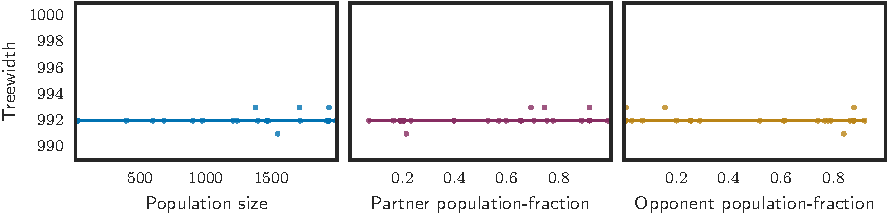
\includegraphics[scale=0.85]{plots/MA1-correlation-regplots-DSJC1000-9-0-crop.pdf}
\vskip 0.5em plus 0.5em minus 0em
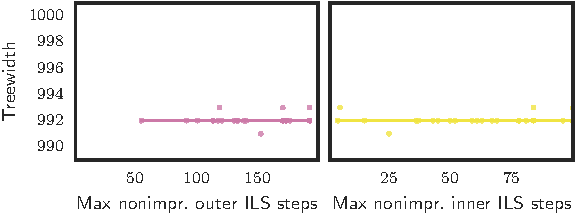
\includegraphics[scale=0.85]{plots/MA1-correlation-regplots-DSJC1000-9-1-crop.pdf}


\caption[Parameter influence for MA1 when applied to \Instance{DSJC1000.9}]{\gls{MA1} applied to \Instance{DSJC1000.9}, 31 samples}

\label{MA1-correlation-regplots-DSJC1000-9}

\end{figure}
\begin{figure}[h]\strictpagecheck\centering

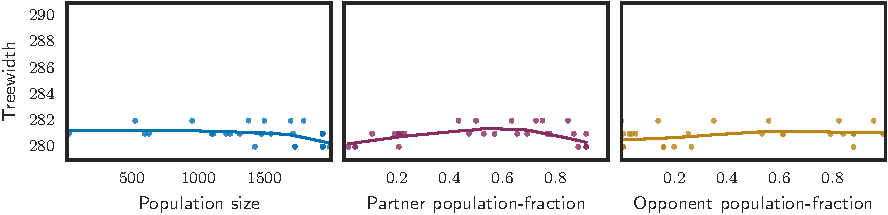
\includegraphics[scale=0.85]{plots/MA1-correlation-regplots-flat300-26-0-0-crop.pdf}
\vskip 0.5em plus 0.5em minus 0em
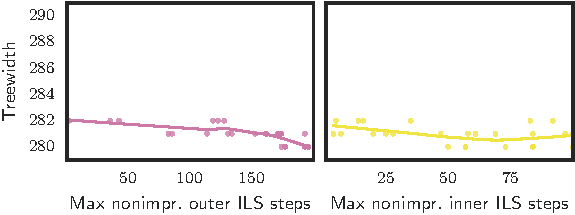
\includegraphics[scale=0.85]{plots/MA1-correlation-regplots-flat300-26-0-1-crop.pdf}


\caption[Parameter influence for MA1 when applied to \Instance{flat300\textunderscore{}26\textunderscore{}0}]{\gls{MA1} applied to \Instance{flat300\textunderscore{}26\textunderscore{}0}, 30 samples}

\label{MA1-correlation-regplots-flat300-26-0}

\end{figure}
\begin{figure}[h]\strictpagecheck\centering

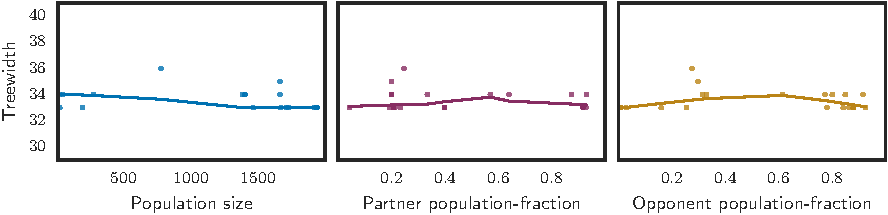
\includegraphics[scale=0.85]{plots/MA1-correlation-regplots-fpsol2-i-2-0-crop.pdf}
\vskip 0.5em plus 0.5em minus 0em
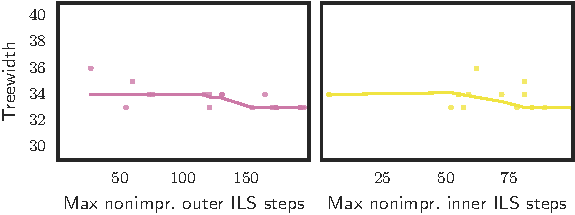
\includegraphics[scale=0.85]{plots/MA1-correlation-regplots-fpsol2-i-2-1-crop.pdf}


\caption[Parameter influence for MA1 when applied to \Instance{fpsol2.i.2}]{\gls{MA1} applied to \Instance{fpsol2.i.2}, 24 samples}

\label{MA1-correlation-regplots-fpsol2-i-2}

\end{figure}
\begin{figure}[h]\strictpagecheck\centering

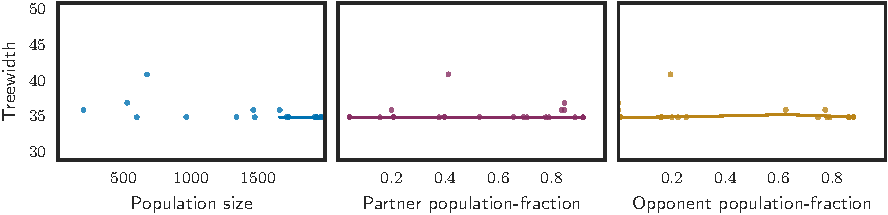
\includegraphics[scale=0.85]{plots/MA1-correlation-regplots-inithx-i-3-0-crop.pdf}
\vskip 0.5em plus 0.5em minus 0em
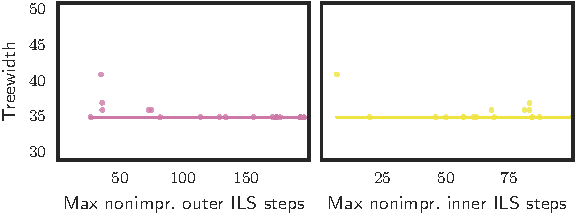
\includegraphics[scale=0.85]{plots/MA1-correlation-regplots-inithx-i-3-1-crop.pdf}


\caption[Parameter influence for MA1 when applied to \Instance{inithx.i.3}]{\gls{MA1} applied to \Instance{inithx.i.3}, 25 samples}

\label{MA1-correlation-regplots-inithx-i-3}

\end{figure}
\begin{figure}[h]\strictpagecheck\centering

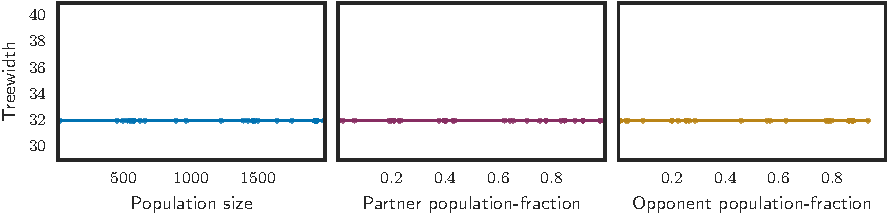
\includegraphics[scale=0.85]{plots/MA1-correlation-regplots-mulsol-i-2-0-crop.pdf}
\vskip 0.5em plus 0.5em minus 0em
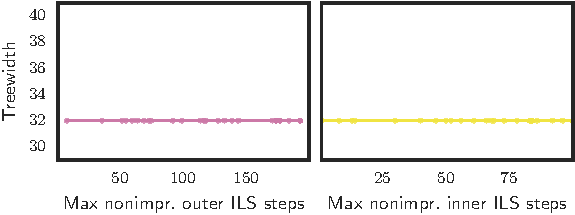
\includegraphics[scale=0.85]{plots/MA1-correlation-regplots-mulsol-i-2-1-crop.pdf}


\caption[Parameter influence for MA1 when applied to \Instance{mulsol.i.2}]{\gls{MA1} applied to \Instance{mulsol.i.2}, 33 samples}

\label{MA1-correlation-regplots-mulsol-i-2}

\end{figure}
\begin{figure}[h]\strictpagecheck\centering

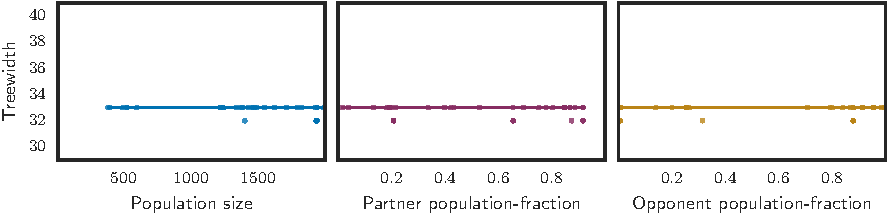
\includegraphics[scale=0.85]{plots/MA1-correlation-regplots-zeroin-i-3-0-crop.pdf}
\vskip 0.5em plus 0.5em minus 0em
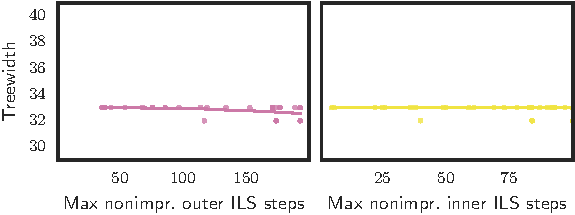
\includegraphics[scale=0.85]{plots/MA1-correlation-regplots-zeroin-i-3-1-crop.pdf}


\caption[Parameter influence for MA1 when applied to \Instance{zeroin.i.3}]{\gls{MA1} applied to \Instance{zeroin.i.3}, 35 samples}

\label{MA1-correlation-regplots-zeroin-i-3}

\end{figure}
\begin{figure}[h]\strictpagecheck\centering

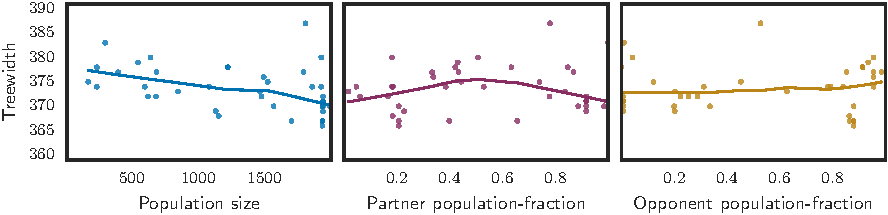
\includegraphics[scale=0.85]{plots/MA1-correlation-regplots-le450-15c-0-crop.pdf}
\vskip 0.5em plus 0.5em minus 0em
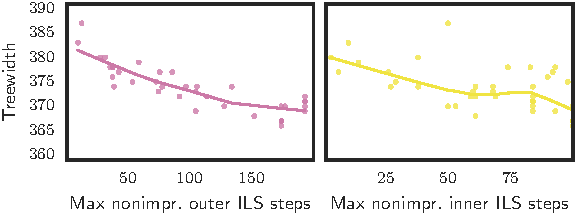
\includegraphics[scale=0.85]{plots/MA1-correlation-regplots-le450-15c-1-crop.pdf}


\caption[Parameter influence for MA1 when applied to \Instance{le450\textunderscore{}15c}]{\gls{MA1} applied to \Instance{le450\textunderscore{}15c}, 38 samples}

\label{MA1-correlation-regplots-le450-15c}

\end{figure}
\begin{figure}[h]\strictpagecheck\centering

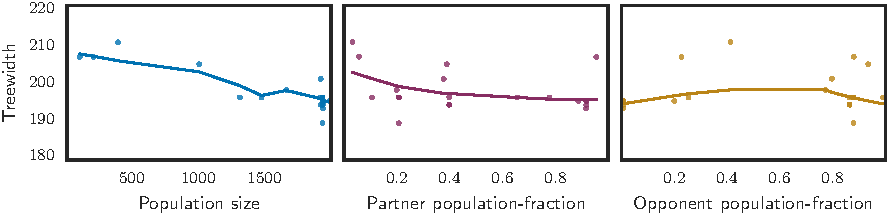
\includegraphics[scale=0.85]{plots/MA1-correlation-regplots-school1-0-crop.pdf}
\vskip 0.5em plus 0.5em minus 0em
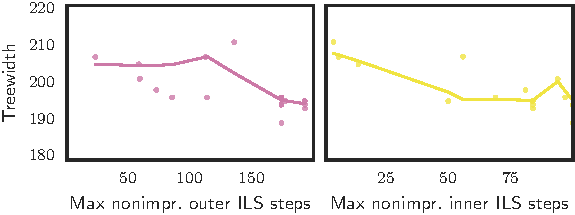
\includegraphics[scale=0.85]{plots/MA1-correlation-regplots-school1-1-crop.pdf}


\caption[Parameter influence for MA1 when applied to \Instance{school1}]{\gls{MA1} applied to \Instance{school1}, 20 samples}

\label{MA1-correlation-regplots-school1}

\end{figure}
\begin{figure}[h]\strictpagecheck\centering

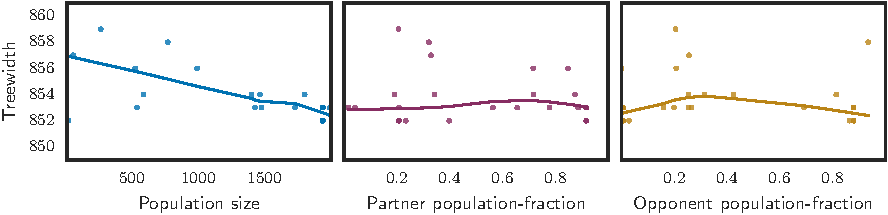
\includegraphics[scale=0.85]{plots/MA1-correlation-regplots-latin-square-10-0-crop.pdf}
\vskip 0.5em plus 0.5em minus 0em
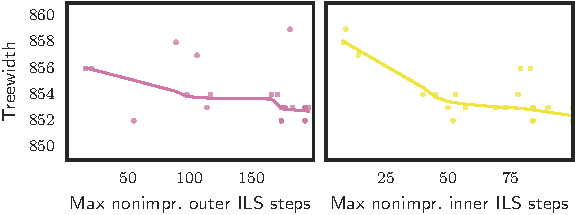
\includegraphics[scale=0.85]{plots/MA1-correlation-regplots-latin-square-10-1-crop.pdf}


\caption[Parameter influence for MA1 when applied to \Instance{latin\textunderscore{}square\textunderscore{}10}]{\gls{MA1} applied to \Instance{latin\textunderscore{}square\textunderscore{}10}, 25 samples}

\label{MA1-correlation-regplots-latin-square-10}

\end{figure}
\begin{figure}[h]\strictpagecheck\centering

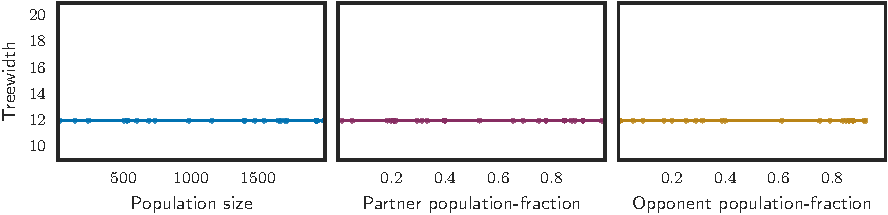
\includegraphics[scale=0.85]{plots/MA1-correlation-regplots-anna-0-crop.pdf}
\vskip 0.5em plus 0.5em minus 0em
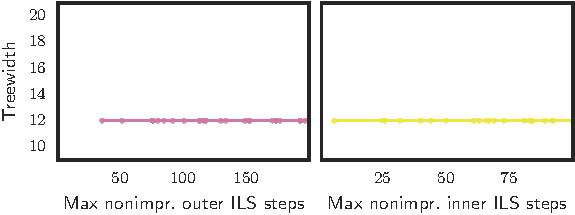
\includegraphics[scale=0.85]{plots/MA1-correlation-regplots-anna-1-crop.pdf}


\caption[Parameter influence for MA1 when applied to \Instance{anna}]{\gls{MA1} applied to \Instance{anna}, 31 samples}

\label{MA1-correlation-regplots-anna}

\end{figure}
\begin{figure}[h]\strictpagecheck\centering

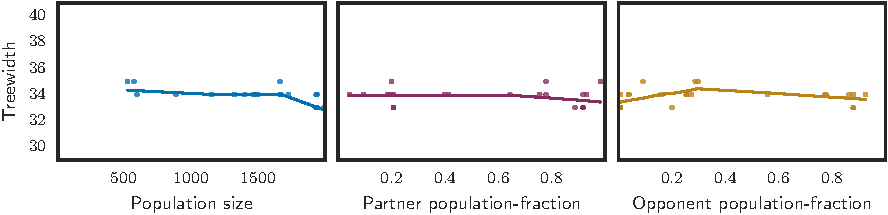
\includegraphics[scale=0.85]{plots/MA1-correlation-regplots-games120-0-crop.pdf}
\vskip 0.5em plus 0.5em minus 0em
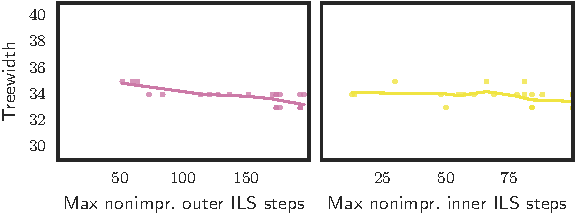
\includegraphics[scale=0.85]{plots/MA1-correlation-regplots-games120-1-crop.pdf}


\caption[Parameter influence for MA1 when applied to \Instance{games120}]{\gls{MA1} applied to \Instance{games120}, 23 samples}

\label{MA1-correlation-regplots-games120}

\end{figure}
\begin{figure}[h]\strictpagecheck\centering

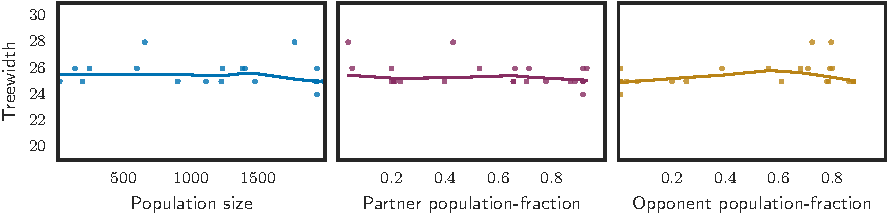
\includegraphics[scale=0.85]{plots/MA1-correlation-regplots-miles500-0-crop.pdf}
\vskip 0.5em plus 0.5em minus 0em
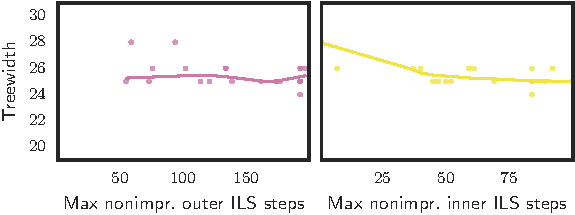
\includegraphics[scale=0.85]{plots/MA1-correlation-regplots-miles500-1-crop.pdf}


\caption[Parameter influence for MA1 when applied to \Instance{miles500}]{\gls{MA1} applied to \Instance{miles500}, 26 samples}

\label{MA1-correlation-regplots-miles500}

\end{figure}
\begin{figure}[h]\strictpagecheck\centering

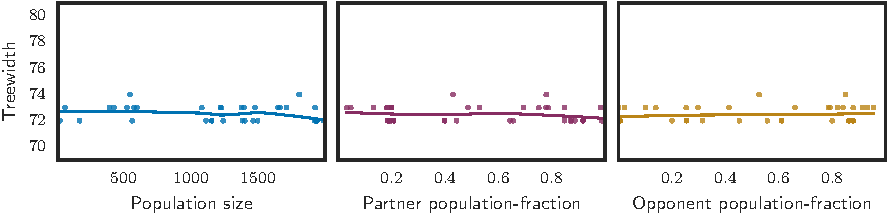
\includegraphics[scale=0.85]{plots/MA1-correlation-regplots-queen10-10-0-crop.pdf}
\vskip 0.5em plus 0.5em minus 0em
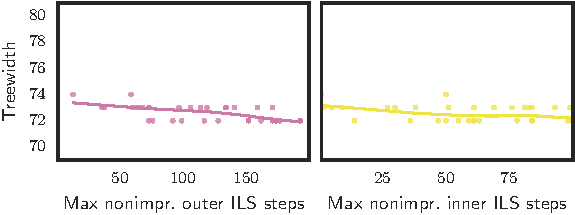
\includegraphics[scale=0.85]{plots/MA1-correlation-regplots-queen10-10-1-crop.pdf}


\caption[Parameter influence for MA1 when applied to \Instance{queen10\textunderscore{}10}]{\gls{MA1} applied to \Instance{queen10\textunderscore{}10}, 41 samples}

\label{MA1-correlation-regplots-queen10-10}

\end{figure}
\begin{figure}[h]\strictpagecheck\centering

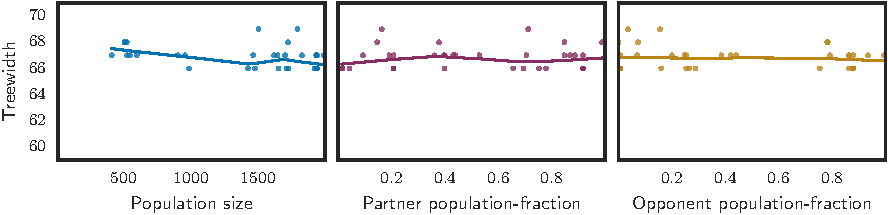
\includegraphics[scale=0.85]{plots/MA1-correlation-regplots-myciel7-0-crop.pdf}
\vskip 0.5em plus 0.5em minus 0em
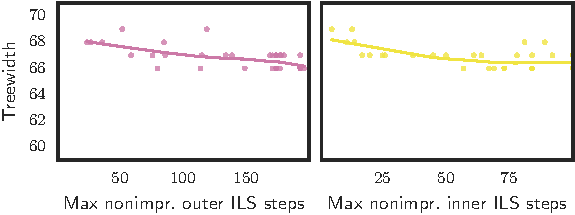
\includegraphics[scale=0.85]{plots/MA1-correlation-regplots-myciel7-1-crop.pdf}


\caption[Parameter influence for MA1 when applied to \Instance{myciel7}]{\gls{MA1} applied to \Instance{myciel7}, 35 samples}

\label{MA1-correlation-regplots-myciel7}

\end{figure}


\clearpage
\subsection{MA2}
%           ^^^
The correlation plots, which are shown in Figures \ref{MA2-correlation-regplots-DSJC500-9} to \ref{MA2-correlation-regplots-myciel6} on pages \pageref{MA2-correlation-regplots-DSJC500-9}--\pageref{MA2-correlation-regplots-myciel6}, do not, for the most part, show any big differences in the impact the individual parameters have on the outcome of the algorithm. Notable exceptions are the instances \Instance{le450\textunderscore{}5c} (Figure~\ref{MA2-correlation-regplots-le450-5c}), \Instance{school1\textunderscore{}nsh} (Figure~\ref{MA2-correlation-regplots-school1-nsh}), \Instance{latin\textunderscore{}square\textunderscore{}10} (Figure~\ref{MA2-correlation-regplots-latin-square-10}), and \Instance{games120} (Figure~\ref{MA2-correlation-regplots-games120}), where the plots clearly affirm \gls{smac}'s results. Interestingly, the crossover parameter, for most instances, does not seem to have as much effect as initially expected.
\begin{figure}[h]\strictpagecheck\centering

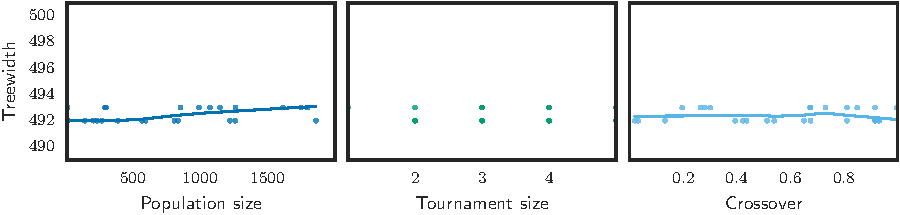
\includegraphics[scale=0.85]{plots/MA2-correlation-regplots-DSJC500-9-0-crop.pdf}
\vskip 0.5em plus 0.5em minus 0em
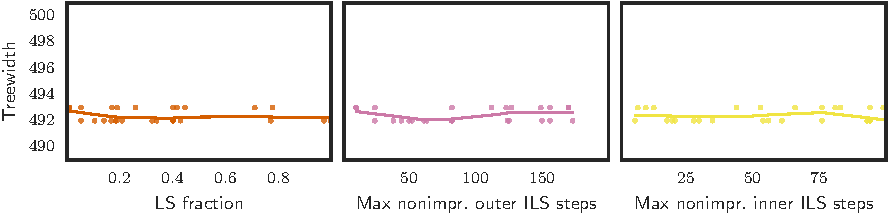
\includegraphics[scale=0.85]{plots/MA2-correlation-regplots-DSJC500-9-1-crop.pdf}


\caption[Parameter influence for MA2 when applied to \Instance{DSJC500.9}]{\gls{MA2} applied to \Instance{DSJC500.9}, 31 samples}

\label{MA2-correlation-regplots-DSJC500-9}

\end{figure}
\begin{figure}[h]\strictpagecheck\centering

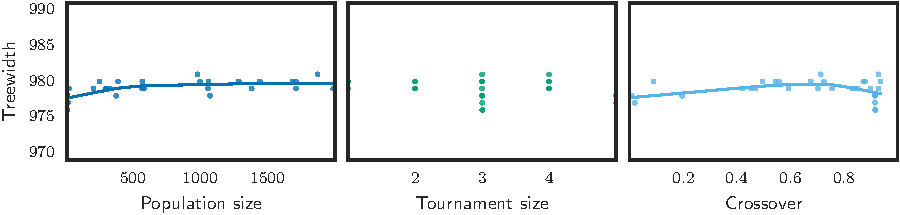
\includegraphics[scale=0.85]{plots/MA2-correlation-regplots-flat1000-76-0-0-crop.pdf}
\vskip 0.5em plus 0.5em minus 0em
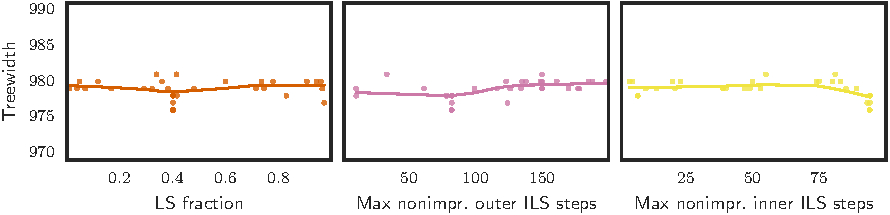
\includegraphics[scale=0.85]{plots/MA2-correlation-regplots-flat1000-76-0-1-crop.pdf}


\caption[Parameter influence for MA2 when applied to \Instance{flat1000\textunderscore{}76\textunderscore{}0}]{\gls{MA2} applied to \Instance{flat1000\textunderscore{}76\textunderscore{}0}, 32 samples}

\label{MA2-correlation-regplots-flat1000-76-0}

\end{figure}
\begin{figure}[h]\strictpagecheck\centering

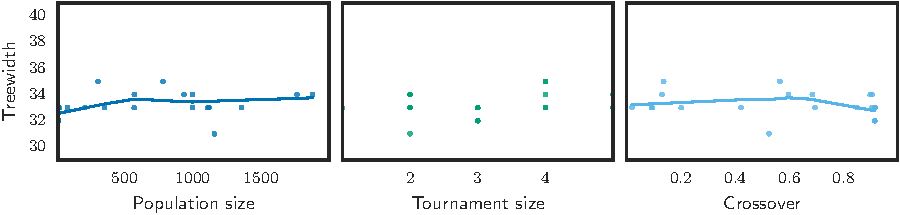
\includegraphics[scale=0.85]{plots/MA2-correlation-regplots-fpsol2-i-3-0-crop.pdf}
\vskip 0.5em plus 0.5em minus 0em
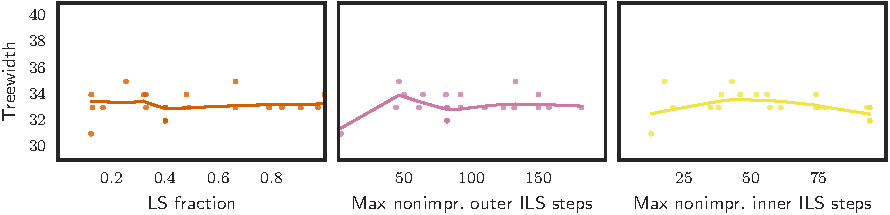
\includegraphics[scale=0.85]{plots/MA2-correlation-regplots-fpsol2-i-3-1-crop.pdf}


\caption[Parameter influence for MA2 when applied to \Instance{fpsol2.i.3}]{\gls{MA2} applied to \Instance{fpsol2.i.3}, 24 samples}

\label{MA2-correlation-regplots-fpsol2-i-3}

\end{figure}
\begin{figure}[h]\strictpagecheck\centering

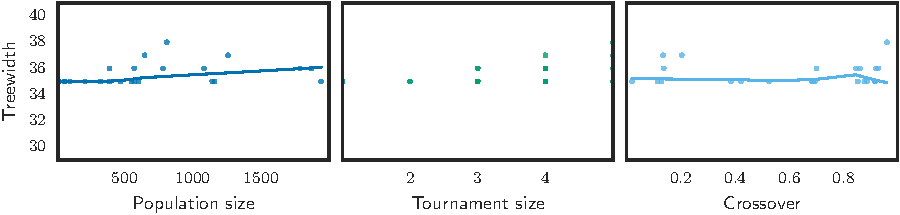
\includegraphics[scale=0.85]{plots/MA2-correlation-regplots-inithx-i-3-0-crop.pdf}
\vskip 0.5em plus 0.5em minus 0em
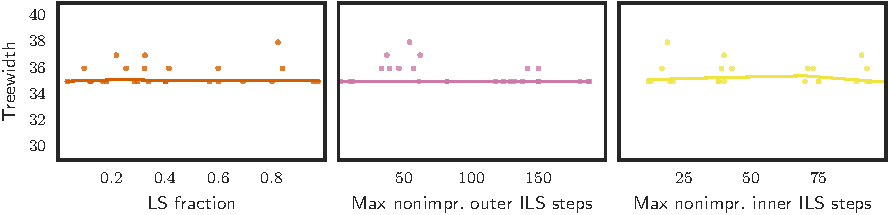
\includegraphics[scale=0.85]{plots/MA2-correlation-regplots-inithx-i-3-1-crop.pdf}


\caption[Parameter influence for MA2 when applied to \Instance{inithx.i.3}]{\gls{MA2} applied to \Instance{inithx.i.3}, 30 samples}

\label{MA2-correlation-regplots-inithx-i-3}

\end{figure}
\begin{figure}[h]\strictpagecheck\centering

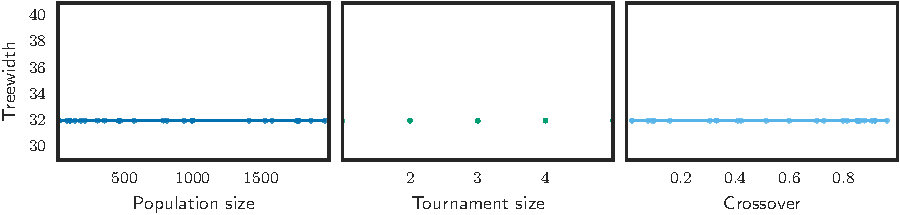
\includegraphics[scale=0.85]{plots/MA2-correlation-regplots-mulsol-i-2-0-crop.pdf}
\vskip 0.5em plus 0.5em minus 0em
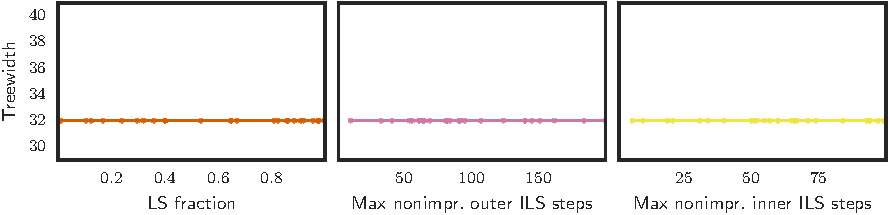
\includegraphics[scale=0.85]{plots/MA2-correlation-regplots-mulsol-i-2-1-crop.pdf}


\caption[Parameter influence for MA2 when applied to \Instance{mulsol.i.2}]{\gls{MA2} applied to \Instance{mulsol.i.2}, 33 samples}

\label{MA2-correlation-regplots-mulsol-i-2}

\end{figure}
\begin{figure}[h]\strictpagecheck\centering

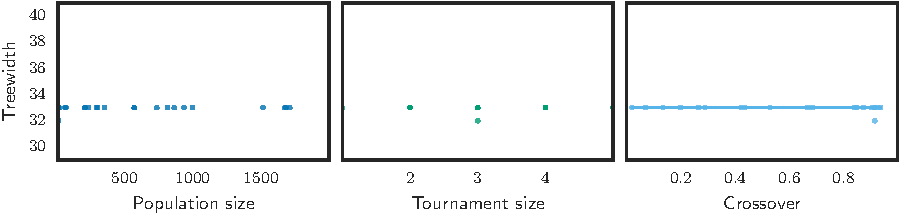
\includegraphics[scale=0.85]{plots/MA2-correlation-regplots-zeroin-i-3-0-crop.pdf}
\vskip 0.5em plus 0.5em minus 0em
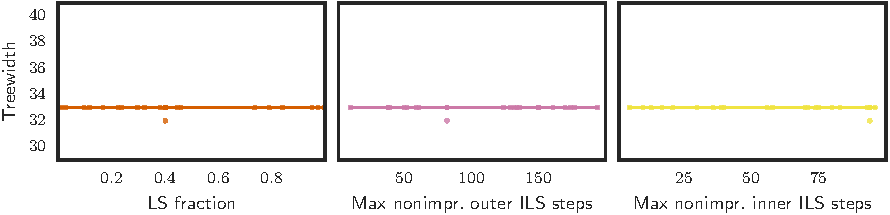
\includegraphics[scale=0.85]{plots/MA2-correlation-regplots-zeroin-i-3-1-crop.pdf}


\caption[Parameter influence for MA2 when applied to \Instance{zeroin.i.3}]{\gls{MA2} applied to \Instance{zeroin.i.3}, 27 samples}

\label{MA2-correlation-regplots-zeroin-i-3}

\end{figure}
\begin{figure}[h]\strictpagecheck\centering

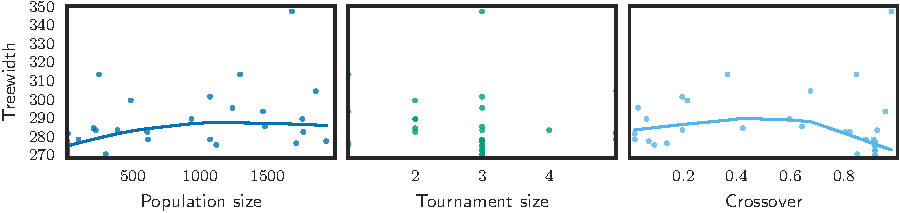
\includegraphics[scale=0.85]{plots/MA2-correlation-regplots-le450-5c-0-crop.pdf}
\vskip 0.5em plus 0.5em minus 0em
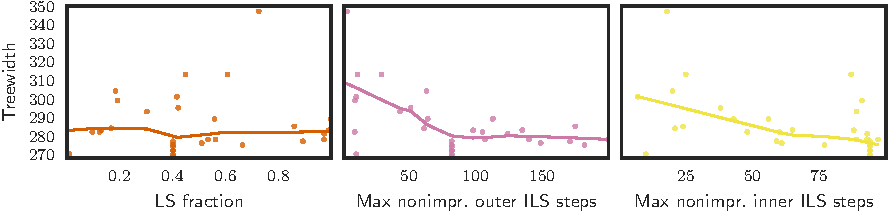
\includegraphics[scale=0.85]{plots/MA2-correlation-regplots-le450-5c-1-crop.pdf}


\caption[Parameter influence for MA2 when applied to \Instance{le450\textunderscore{}5c}]{\gls{MA2} applied to \Instance{le450\textunderscore{}5c}, 31 samples}

\label{MA2-correlation-regplots-le450-5c}

\end{figure}
\begin{figure}[h]\strictpagecheck\centering

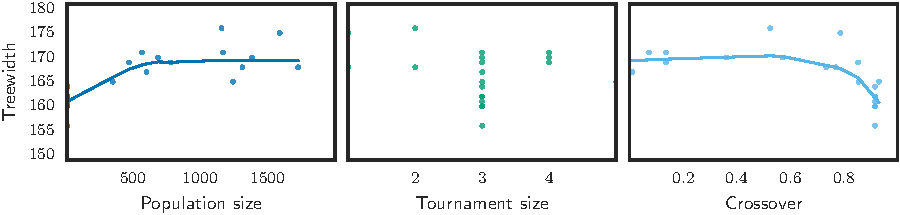
\includegraphics[scale=0.85]{plots/MA2-correlation-regplots-school1-nsh-0-crop.pdf}
\vskip 0.5em plus 0.5em minus 0em
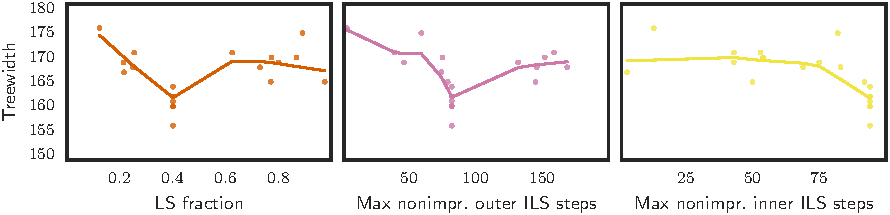
\includegraphics[scale=0.85]{plots/MA2-correlation-regplots-school1-nsh-1-crop.pdf}


\caption[Parameter influence for MA2 when applied to \Instance{school1\textunderscore{}nsh}]{\gls{MA2} applied to \Instance{school1\textunderscore{}nsh}, 20 samples}

\label{MA2-correlation-regplots-school1-nsh}

\end{figure}
\begin{figure}[h]\strictpagecheck\centering

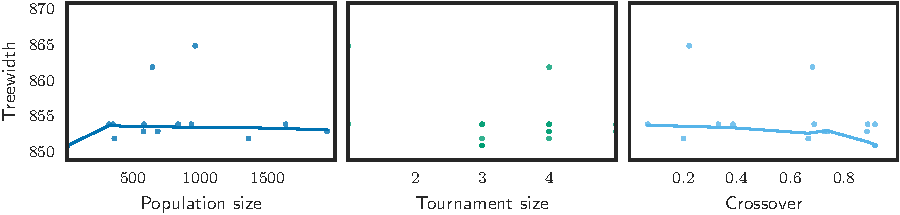
\includegraphics[scale=0.85]{plots/MA2-correlation-regplots-latin-square-10-0-crop.pdf}
\vskip 0.5em plus 0.5em minus 0em
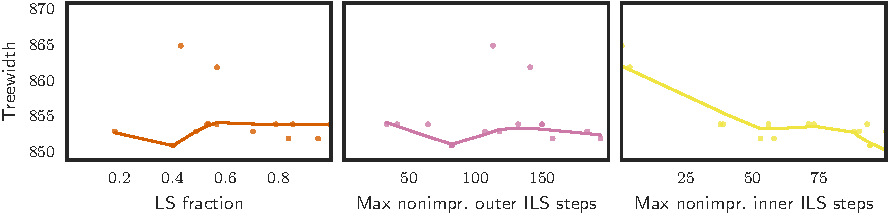
\includegraphics[scale=0.85]{plots/MA2-correlation-regplots-latin-square-10-1-crop.pdf}


\caption[Parameter influence for MA2 when applied to \Instance{latin\textunderscore{}square\textunderscore{}10}]{\gls{MA2} applied to \Instance{latin\textunderscore{}square\textunderscore{}10}, 20 samples}

\label{MA2-correlation-regplots-latin-square-10}

\end{figure}
\begin{figure}[h]\strictpagecheck\centering

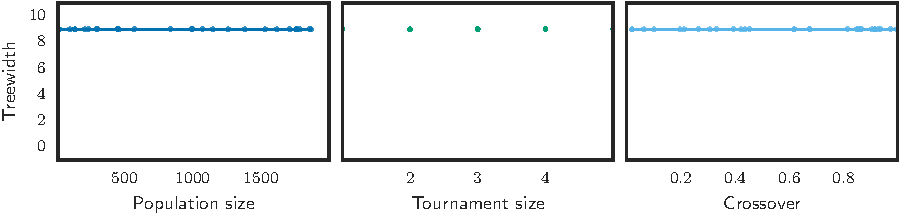
\includegraphics[scale=0.85]{plots/MA2-correlation-regplots-jean-0-crop.pdf}
\vskip 0.5em plus 0.5em minus 0em
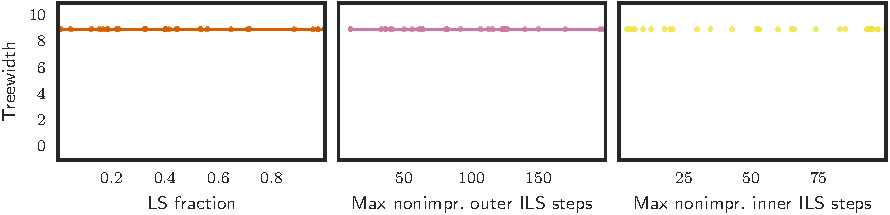
\includegraphics[scale=0.85]{plots/MA2-correlation-regplots-jean-1-crop.pdf}


\caption[Parameter influence for MA2 when applied to \Instance{jean}]{\gls{MA2} applied to \Instance{jean}, 35 samples}

\label{MA2-correlation-regplots-jean}

\end{figure}
\begin{figure}[h]\strictpagecheck\centering

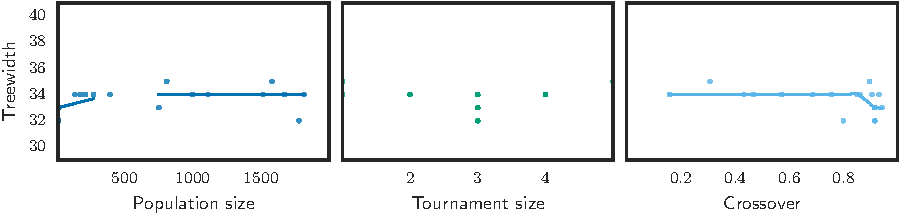
\includegraphics[scale=0.85]{plots/MA2-correlation-regplots-games120-0-crop.pdf}
\vskip 0.5em plus 0.5em minus 0em
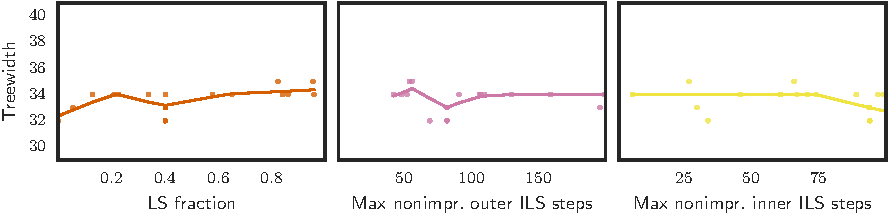
\includegraphics[scale=0.85]{plots/MA2-correlation-regplots-games120-1-crop.pdf}


\caption[Parameter influence for MA2 when applied to \Instance{games120}]{\gls{MA2} applied to \Instance{games120}, 22 samples}

\label{MA2-correlation-regplots-games120}

\end{figure}
\begin{figure}[h]\strictpagecheck\centering

\includegraphics[scale=0.85]{plots/MA2-correlation-regplots-miles1000-0-crop.pdf}
\vskip 0.5em plus 0.5em minus 0em
\includegraphics[scale=0.85]{plots/MA2-correlation-regplots-miles1000-1-crop.pdf}


\caption[Parameter influence for MA2 when applied to \Instance{miles1000}]{\gls{MA2} applied to \Instance{miles1000}, 28 samples}

\label{MA2-correlation-regplots-miles1000}

\end{figure}
\begin{figure}[h]\strictpagecheck\centering

\includegraphics[scale=0.85]{plots/MA2-correlation-regplots-queen12-12-0-crop.pdf}
\vskip 0.5em plus 0.5em minus 0em
\includegraphics[scale=0.85]{plots/MA2-correlation-regplots-queen12-12-1-crop.pdf}


\caption[Parameter influence for MA2 when applied to \Instance{queen12\textunderscore{}12}]{\gls{MA2} applied to \Instance{queen12\textunderscore{}12}, 31 samples}

\label{MA2-correlation-regplots-queen12-12}

\end{figure}
\begin{figure}[h]\strictpagecheck\centering

\includegraphics[scale=0.85]{plots/MA2-correlation-regplots-myciel6-0-crop.pdf}
\vskip 0.5em plus 0.5em minus 0em
\includegraphics[scale=0.85]{plots/MA2-correlation-regplots-myciel6-1-crop.pdf}


\caption[Parameter influence for MA2 when applied to \Instance{myciel6}]{\gls{MA2} applied to \Instance{myciel6}, 32 samples}

\label{MA2-correlation-regplots-myciel6}

\end{figure}


\clearpage
\subsection{MA3}
%           ^^^
Correlation plots for \gls{MA3} are shown in Figures \ref{MA3-correlation-regplots-DSJR500-1c} to \ref{MA3-correlation-regplots-myciel6} on pages \pageref{MA3-correlation-regplots-DSJR500-1c}--\pageref{MA3-correlation-regplots-myciel6}.

For \enquote{simple} instances like \Instance{mulsol.i.1}, \Instance{zeroin.i.3}, \Instance{jean}, or \Instance{myciel6}, it seems that the parameter settings do not influence the result at all. The plots for the other instances show more variety. The population size parameter seems to induce good performance when chosen to be either low or high, but appears to have a negative impact over the remaining part of the spectrum. Lower is better seems to be true for the maximal number of nonimproving outer steps, albeit there is a trend for higher values to again improve results a bit.
\begin{figure}[h]\strictpagecheck\centering

\includegraphics[scale=0.85]{plots/MA3-correlation-regplots-DSJR500-1c-0-crop.pdf}


\caption[Parameter influence for MA3 when applied to \Instance{DSJR500.1c}]{\gls{MA3} applied to \Instance{DSJR500.1c}, 39 samples}

\label{MA3-correlation-regplots-DSJR500-1c}

\end{figure}
\begin{figure}[h]\strictpagecheck\centering

\includegraphics[scale=0.85]{plots/MA3-correlation-regplots-flat300-26-0-0-crop.pdf}


\caption[Parameter influence for MA3 when applied to \Instance{flat300\textunderscore{}26\textunderscore{}0}]{\gls{MA3} applied to \Instance{flat300\textunderscore{}26\textunderscore{}0}, 32 samples}

\label{MA3-correlation-regplots-flat300-26-0}

\end{figure}
\begin{figure}[h]\strictpagecheck\centering

\includegraphics[scale=0.85]{plots/MA3-correlation-regplots-fpsol2-i-3-0-crop.pdf}


\caption[Parameter influence for MA3 when applied to \Instance{fpsol2.i.3}]{\gls{MA3} applied to \Instance{fpsol2.i.3}, 27 samples}

\label{MA3-correlation-regplots-fpsol2-i-3}

\end{figure}
\begin{figure}[h]\strictpagecheck\centering

\includegraphics[scale=0.85]{plots/MA3-correlation-regplots-inithx-i-3-0-crop.pdf}


\caption[Parameter influence for MA3 when applied to \Instance{inithx.i.3}]{\gls{MA3} applied to \Instance{inithx.i.3}, 25 samples}

\label{MA3-correlation-regplots-inithx-i-3}

\end{figure}
\begin{figure}[h]\strictpagecheck\centering

\includegraphics[scale=0.85]{plots/MA3-correlation-regplots-mulsol-i-1-0-crop.pdf}


\caption[Parameter influence for MA3 when applied to \Instance{mulsol.i.1}]{\gls{MA3} applied to \Instance{mulsol.i.1}, 33 samples}

\label{MA3-correlation-regplots-mulsol-i-1}

\end{figure}
\begin{figure}[h]\strictpagecheck\centering

\includegraphics[scale=0.85]{plots/MA3-correlation-regplots-zeroin-i-3-0-crop.pdf}


\caption[Parameter influence for MA3 when applied to \Instance{zeroin.i.3}]{\gls{MA3} applied to \Instance{zeroin.i.3}, 31 samples}

\label{MA3-correlation-regplots-zeroin-i-3}

\end{figure}
\begin{figure}[h]\strictpagecheck\centering

\includegraphics[scale=0.85]{plots/MA3-correlation-regplots-le450-15c-0-crop.pdf}


\caption[Parameter influence for MA3 when applied to \Instance{le450\textunderscore{}15c}]{\gls{MA3} applied to \Instance{le450\textunderscore{}15c}, 34 samples}

\label{MA3-correlation-regplots-le450-15c}

\end{figure}
\begin{figure}[h]\strictpagecheck\centering

\includegraphics[scale=0.85]{plots/MA3-correlation-regplots-school1-0-crop.pdf}


\caption[Parameter influence for MA3 when applied to \Instance{school1}]{\gls{MA3} applied to \Instance{school1}, 23 samples}

\label{MA3-correlation-regplots-school1}

\end{figure}
\begin{figure}[h]\strictpagecheck\centering

\includegraphics[scale=0.85]{plots/MA3-correlation-regplots-latin-square-10-0-crop.pdf}


\caption[Parameter influence for MA3 when applied to \Instance{latin\textunderscore{}square\textunderscore{}10}]{\gls{MA3} applied to \Instance{latin\textunderscore{}square\textunderscore{}10}, 26 samples}

\label{MA3-correlation-regplots-latin-square-10}

\end{figure}
\begin{figure}[h]\strictpagecheck\centering

\includegraphics[scale=0.85]{plots/MA3-correlation-regplots-jean-0-crop.pdf}


\caption[Parameter influence for MA3 when applied to \Instance{jean}]{\gls{MA3} applied to \Instance{jean}, 37 samples}

\label{MA3-correlation-regplots-jean}

\end{figure}
\begin{figure}[h]\strictpagecheck\centering

\includegraphics[scale=0.85]{plots/MA3-correlation-regplots-games120-0-crop.pdf}


\caption[Parameter influence for MA3 when applied to \Instance{games120}]{\gls{MA3} applied to \Instance{games120}, 21 samples}

\label{MA3-correlation-regplots-games120}

\end{figure}
\begin{figure}[h]\strictpagecheck\centering

\includegraphics[scale=0.85]{plots/MA3-correlation-regplots-miles500-0-crop.pdf}


\caption[Parameter influence for MA3 when applied to \Instance{miles500}]{\gls{MA3} applied to \Instance{miles500}, 23 samples}

\label{MA3-correlation-regplots-miles500}

\end{figure}
\begin{figure}[h]\strictpagecheck\centering

\includegraphics[scale=0.85]{plots/MA3-correlation-regplots-queen10-10-0-crop.pdf}


\caption[Parameter influence for MA3 when applied to \Instance{queen10\textunderscore{}10}]{\gls{MA3} applied to \Instance{queen10\textunderscore{}10}, 32 samples}

\label{MA3-correlation-regplots-queen10-10}

\end{figure}
\begin{figure}[h]\strictpagecheck\centering

\includegraphics[scale=0.85]{plots/MA3-correlation-regplots-myciel6-0-crop.pdf}


\caption[Parameter influence for MA3 when applied to \Instance{myciel6}]{\gls{MA3} applied to \Instance{myciel6}, 30 samples}

\label{MA3-correlation-regplots-myciel6}

\end{figure}





\end{document}
% vim: set ts=3 sts=3 sw=3 tw=0 et :
